\section{Vector Function}

So far, we have considered multi-variable functions. The function takes in 2 (or 3) inputs, and gives out 1 output:
$$f(x, y): \mathbb{R}^2 \to \mathbb{R}$$
$$f(x, y, z): \mathbb{R}^3 \to \mathbb{R}$$

We can also have \term{vector functions}\index{Vector Function}, which gives \bred{multiple outputs}. In general, we can have $$\begin{matrix} f: &\mathbb{R}^m &\to &\mathbb{R}^n \\ &\begin{bmatrix} x_1 \\ x_2 \\ x_3 \\ \vdots \\ x_m \end{bmatrix} &\mapsto &\begin{bmatrix} y_1 \\ y_2 \\ \vdots \\ y_n \end{bmatrix} \end{matrix}$$ It is called a vector function, since $f$ have many outputs, so the outputs as a whole can be regarded as a vector. $$f(\vec{x}) = \vec{y}$$

Each output may depend on \bred{all of the inputs}, and so each output is a \term{coordinate function}\index{Coordinate Function} that depends on all of the input variables. In other words, a vector function is made up of many multi-variable functions. $$f\begin{pmatrix}
        x_1 \\ x_2 \\ x_3 \\ \vdots \\ x_m
    \end{pmatrix} = \begin{bmatrix}
        f_1(x_1, x_2, x_3, \cdots, x_m) \\
        f_2(x_1, x_2, x_3, \cdots, x_m) \\
        \vdots                          \\
        f_n(x_1, x_2, x_3, \cdots, x_m) \\
    \end{bmatrix} = \begin{bmatrix}
        y_1 \\ y_2 \\ \vdots \\ y_n
    \end{bmatrix}$$

This makes extending the definitions from multi-variable functions to vector functions very easy. 

\begin{definition}
    A vector function f is integrable/continuous/differentiable, when all of its coordinate functions are integrable/continuous/differentiable.
\end{definition}

If we focus only within 3 dimensions, there are (mainly) 2 new types of functions.

\section{Parametrization}

\begin{definition}[Parametrization]\index{Parametrization}
    When $f$ goes from a lower dimensional space, to a higher dimensional space, we sometimes call f a \term{parametrization}.
\end{definition}

\subsection*{1D Parametrization}

$$f(t): \mathbb{R} \to \mathbb{R}^2 \qquad \text{\textbf{OR}} \qquad f(t): \mathbb{R} \to \mathbb{R}^3$$ where we have used the variable $t$ as the input of $f$.

Thus, for each $t$, $f(t) = (x, y)$ is a point in 2D, or $f(t) = (x, y, z)$ in 3D.

If we view $t$ as time, then we can view $f(t)$ as the position of an object. Thus $f(t)$ describes the position of an object, as time goes on, which will traverse out a curve. Since a curve is a 1D object, this is called a \term{1D parametrization}.

In fact, this is one of the most important ways to describe a curve in higher dimensions, and finding a parametrization for a given curve is an important skill in Calculus.

\begin{example}
    Given a circle of radius $R$ at the origin, we can choose the parametrization to be $$f(t) = (R \cos{t}, R \sin{t}) = (x, y) \qquad t\in [0, 2\pi]$$ where $x = R \cos{t}$, $y = R \sin{t}$ is not the standard polar coordinates.

    The parametrization starts at $t = 0$, which is the point $(0, R)$. Then as $t$ increases, $f(t)$ traverses the circle clockwise, since $t$ is now the angle between the point $(x, y)$ and the positive $y$-axis.

    We still traverse the whole circle, but this is the less natural parametrization.

    \begin{minipage}{0.45\linewidth}
        \begin{center}
            \def\arraystretch{2}
            \begin{tabular}{c|c}
                t & $(x,y)$ \\
                \hline
                $0$ & $(0,R)$ \\
                $\frac{\pi}{2}$ & $(R,0)$ \\
                $\pi$ & $(0,-R)$ \\
                $\frac{3\pi}{2}$ & $(-R,0)$ \\
            \end{tabular}
        \end{center}
    \end{minipage}
    \begin{minipage}{0.45\linewidth}
        \begin{center}
            \tikzsetnextfilename{c05s02-f01}%
            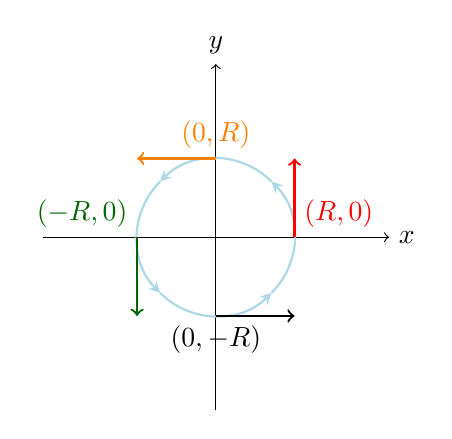
\begin{tikzpicture}
                \draw[->] (-2.2,0) -- (2.2,0) node[right] {$x$};
                \draw[->] (0,-2.2) -- (0,2.2) node[above] {$y$};
            
                \draw[thick,LightBlue,-stealth] (0.7071,0.7071) arc(45:135:1);
                \draw[thick,LightBlue,-stealth] (-0.7071,0.7071) arc(135:225:1);
                \draw[thick,LightBlue,-stealth] (-0.7071,-0.7071) arc(225:315:1);
                \draw[thick,LightBlue,-stealth] (0.7071,-0.7071) arc(-45:45:1);
            
                \node[red,above right] at (1,0) {$(R,0)$};
                \draw[thick,red,->] (1,0) -- (1,1);
                \node[orange,above] at (0,1) {$(0,R)$};
                \draw[thick,orange,->] (0,1) -- (-1,1);
                \node[DarkGreen,above left] at (-1,0) {$(-R,0)$};
                \draw[thick,DarkGreen,->] (-1,0) -- (-1,-1);
                \node[below] at (0,-1) {$(0,-R)$};
                \draw[thick,->] (0,-1) -- (1,-1);
            \end{tikzpicture}
        \end{center}
    \end{minipage}
\end{example}

When we need a parametrization of a curve, we typically choose the easiest one.

\subsection*{2D Parametrization}

$$f(u, v): \mathbb{R}^2 \to \mathbb{R}^3$$ where we have used the variables $u, v$ as the inputs of $f$. Thus for each $(u, v)$ in 2D, $f(u, v) = (x, y, z)$ is a point in 3D. 

Given a 2D region in the domain $\mathbb{R}^2$ (such as a square), $f(u, v)$ will create a surface in 3D. Since a surface is a 2D object, this is called a \term{2D parametrization}. 

\begin{itemize}
    \item Going from left to right, we may think that $f$ lifts up a 2D region in $\mathbb{R}^2$ into 3D, and maybe stretches the region somewhat, depending on the definition of $f$.
    
    \item Going from right to left, given a surface $S$ in 3D, we can try to find a parametrization for this surface $f(u, v) = (x, y, z)$. $f$ pulls back this (curved) surface $S$ in 3D with $(x, y, z)$ as variables, into a flat region in 2D with $(u, v)$ as variables.
\end{itemize}

We know that an equality involving $x$, $y$, $z$ gives a surface in 3D: $g(x, y, z) = 0$. This gives an alternative way of describing a surface in 3D. Finding a parametrization for a given surface is also an important skill in Calculus.

\begin{example}
    If we consider the plane $z = x + y + 10$ that is above the unit square on the $xy$-plane, we may choose the parametrization to be $$f(u, v) = (u, v, u + v + 10) = (x, y, z) \qquad u \in [0, 1] \qquad v \in [0, 1]$$

    This is called the natural parametrization, as we have set $u = x$ and $v = y$. For any point $(x, y) = (u, v)$ on the $xy$-plane, $f$ takes in this point, and gives out the same point with a new 3rd coordinate, or height, with the 3rd component defined by $f: z = u + v + 10$.

    This \itblue{lifts up} the unit square from the $xy$-plane, onto the plane $z = x + y + 10$. However, notice that the square is now slanted, and also stretched. In this case, the plane $z = x + y + 10$ is flat, but in general, $f$ lifts up a flat region in 2D, into a curved surface in 3D, with some stretching.
    
    \begin{minipage}{0.45\linewidth}
        \begin{center}
            \tikzsetnextfilename{c05s02-f02}%
            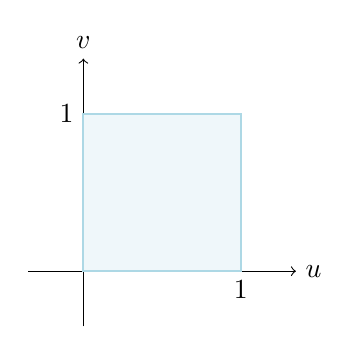
\begin{tikzpicture}
                \draw[->] (-0.7,0) -- (2.7,0) node[right] {$u$};
                \draw[->] (0,-0.7) -- (0,2.7) node[above] {$v$};

                \draw[thick,LightBlue,fill=LightBlue,fill opacity=0.2] (0,0) -- (0,2) -- (2,2) -- (2,0) -- cycle;

                \node[below] at(2,0) {$1$};
                \node[left] at(0,2) {$1$};
            \end{tikzpicture}
        \end{center}
    \end{minipage}
    \begin{minipage}{0.45\linewidth}
        \begin{center} \includegraphics[width=0.95\linewidth]{Plots/s_5_2/u_v_uv10.png} \end{center}
    \end{minipage}

    In reverse, we can view $f$ pulls back a (possibly complicated) surface in 3D, (in this case $z = x + y + 10$), into a flat region in 2D (the unit square).
\end{example}

\section{Coordinate Transformation}

\begin{definition}[Coordinate Transformation]\index{Coordinate Transformation}
    When $f$ goes between spaces of the same dimension, we sometimes call $f$ a \term{coordinate transformation}. 

    $$f(u, v): \mathbb{R}^2 \to \mathbb{R}^2 \qquad \textbf{OR} \qquad f(u, v, w): \mathbb{R}^3 \to \mathbb{R}^3$$ where $f(u, v) = (x, y)$, and $f(u, v, w) = (x, y, z)$.
\end{definition}

\begin{itemize}
    \item Going from left to right, given a 2D region in the domain $\mathbb{R}^2$ (such as a square), $f(u, v) = (x, y)$ will produce another 2D region in $\mathbb{R}^2$, with some stretching as defined by $f$.

    \item Going from right to left, given a (possibly complicated) region in 2D with variables $(x, y)$, we can try to find a coordinate transformation $f$ for this region, where $f(u, v)$ transforms a simple region in the $uv$-plane, onto the original region in the $xy$-plane.
\end{itemize}

We have found a new set of coordinates $(u, v)$, to describe the more complicated region in the $xy$-plane.

Similarly, we can also do this for regions in 3D.

\begin{example}
    Given a \bred{solid} circle of radius $R$ at the origin, $x^2 + y^2 \le R^2$, it is a region in 2D. We know that representing this region is complicated in $(x, y)$, where we get expressions such as $y = \sqrt{R^2 - x^2}$.

    However, we may consider \term{polar coordinates}: $$f(r,\theta) = (r\cos{\theta},r\sin{\theta}) = (x,y) \qquad r \in [0,R] \qquad \theta \in [0,2\pi]$$ where for each point $(r,\theta)$ in the ``$r - \theta$'' plane, $f(r,\theta) = (x,y)$ is a point in the solid circle in the $xy$-plane.

    In other words, $f$ transforms a solid rectangle in the ``$r - \theta$'' plane, into the solid circle in the $xy$-plane. Instead of working with a circle, we now can work with a rectangle instead, as we have found \bred{better coordinates} to describe the original region in the $xy$-plane.
\end{example}

For $f$ to turn a rectangle into a circle, it must stretch the rectangle at multiple places, at different rates, which is based on the definition of $f$.

\section{Derivative Matrix}

Given a vector function, for example $f(x,y,z)$, $$f\begin{bmatrix} x \\ y \\ z \end{bmatrix} = \begin{bmatrix} f_1(x,y,z) \\ f_2(x,y,z) \\ f_3(x,y,z) \end{bmatrix}$$

The derivative of a vector function is $D_f$, called the derivative matrix.

For the first row of the matrix, we take the first coordinate function, and take the partial derivative with respect to all possible variables $(x,y,z)$ \bred{in order}, horizontally. Then for each coordinate function, we do the same thing to get a new row of the matrix. 

$$D_f = \begin{bmatrix}
    \frac{\partial}{\partial x} f_1 & \frac{\partial}{\partial y} f_1 & \frac{\partial}{\partial z} f_1 \\
    \frac{\partial}{\partial x} f_2 & \frac{\partial}{\partial y} f_2 & \frac{\partial}{\partial z} f_2 \\
    \frac{\partial}{\partial x} f_3 & \frac{\partial}{\partial y} f_3 & \frac{\partial}{\partial z} f_3 \\
\end{bmatrix}$$

\subsection*{Relation to Gradient $\nabla f$}

For a multi-variable function $f(x, y, z): \mathbb{R}^3 \to \mathbb{R}$, it returns one value (for example, $f(x,y,z) = xyz^2$). $$D_f = \nabla f = (\frac{\partial}{\partial x} f, \frac{\partial}{\partial y} f, \frac{\partial}{\partial z} f)$$ where the derivative matrix has only 1 row. 

On the other hand, for a vector function: $f(x, y, z) = (f_1, f_2, f_3)$, each row
of Df is the gradient of all the coordinate functions: $$D_f = \begin{bmatrix} - \nabla f_1 - \\ - \nabla f_2 - \\ - \nabla f_3 - \end{bmatrix}$$ where $\nabla f_i$ are viewed as horizontal vectors in the matrix.

\begin{exercise}
    $$f(x, y, z) = (3x + y, e^yz, xyz)$$

    First, state the dimension of the vector $f$ takes in, and the dimension of the vector $f$ gives out. Then, compute $D_f$.
\end{exercise}

\section{Change of Variable Formula}

Suppose you need to integrate $f$ over a domain $B$, but $B$ is very bad, You don't want to integrate over a bad domain. Suppose you can find a function $g$ such that $g$ takes another region a onto B. $$g: A \to B \qquad g(A) = B$$ and somehow $A$ is good domain. 

So, instead of integrating $f$ over the bad domain $B$, you can integrate over the good domain $A$ instead. $$\int_B f = \int_A f \circ g \cdot \left| \det(D_g) \right|$$ $f \circ g$ means replacing the old variables of $f$ in $B$ with the new ones in $A$ (we require that $g$ to be a one-to-one transformation, and $\det(D_g) \neq 0)$. The natural question is of course: How do I find such $g$?

\subsection*{Polar Coordinates}

Need to integrate $f(x, y)$. 
$$g(r,\theta) = (r\cos{\theta},r\sin{\theta}) = (x,y)$$

$f \circ g = f(g(r, \theta)) = f(r\cos{\theta}, r\sin{\theta}) = f(x, y)$ and $r^2 = x^2 + y^r$. 
$$\det(D_f) = r$$

Useful when domain $B$ is (partly) of circular shape, or function given is already in polar coordinates.

\begin{exercise}
    Integrate $f(x,y) = x$ over $D = {1 \le x^2 + y^2 \le 4}$ in the 2nd quadrant.
\end{exercise}

\begin{exercise}
    Show that $\int_{-\infty}^{+\infty} e^{-x^2} \,dx = \sqrt{\pi}$

    \textbf{Strategy: } The normal distribution has no anti-derivative. Start with $\left( \int_{-\infty}^{+\infty} e^{-x^2} \right)^2$ and write it as a product of 2 same things. Then change the variable in one integral from $x$ to $y$, and use the polar coordinate transformation.
\end{exercise}